\documentclass{article}
\usepackage{tikz}
\usetikzlibrary{intersections}
\usetikzlibrary{calc}
\usetikzlibrary {arrows.meta}

\begin{document}

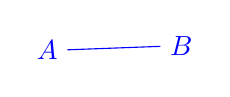
\begin{tikzpicture}
  \coordinate [label=left:\textcolor{blue}{$A$}]  (A) at ($(0,0 + .1*(rand,rand)$);
  \coordinate [label=right:\textcolor{blue}{$B$}] (B) at ($(1.25,0.25) + .1*(rand,rand)$);

  \draw[blue] (A) -- (B);


\end{tikzpicture}

  \foreach \x in {1,...,10}{\pgfmathparse{rand}\pgfmathresult, }

\end{document}
